% generated by scripts/pkl_to_latex.py
% source PKL : tscan_v1_L6_Ne5_U10_mode-uniform_nmin2_solver-gcg_full_restarts10_iter300_kmax4_tol1em09_t0.05to2_N20-d03538a42051.pkl
% scan type  : tscan
% state      : gs
% requires   : \usepackage{pgfplots} \pgfplotsset{compat=1.18}
% colours match the matplotlib PDF (tab10 cycle)
\definecolor{gmeC0}{HTML}{1F77B4}
\definecolor{gmeC1}{HTML}{FF7F0E}
\definecolor{gmeC2}{HTML}{2CA02C}
\definecolor{gmeC3}{HTML}{D62728}
\definecolor{gmeC4}{HTML}{9467BD}
\definecolor{gmeC5}{HTML}{8C564B}
\definecolor{gmeC6}{HTML}{E377C2}
\definecolor{gmeC7}{HTML}{17BECF}

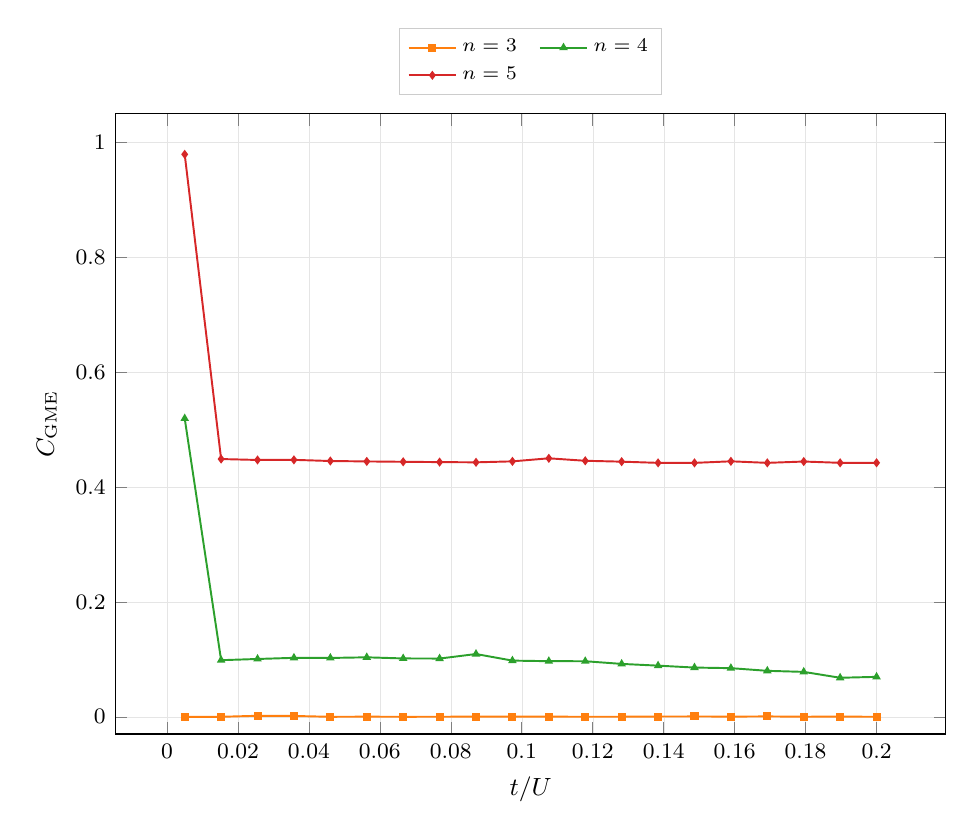
\begin{tikzpicture}
  \begin{axis}[
    width=\columnwidth,
    height=0.78\columnwidth,
    xlabel={$t/U$},
    ylabel={$C_{\mathrm{GME}}$},
    grid=both,
    grid style={line width=.1pt, draw=gray!20},
    tick label style={font=\footnotesize\rmfamily, /pgf/number format/fixed},
    label style={font=\small\rmfamily},
    scaled ticks=false,
    legend style={font=\scriptsize\rmfamily, draw=gray!40, at={(0.5,1.03)}, anchor=south, /tikz/every even column/.append style={column sep=6pt}},
    legend cell align={left},
    legend columns=2,
    ymin=-0.03,
    ymax=1.05,
  ]
    \addplot[color=gmeC1, mark=square*, mark size=1.1pt, line width=0.7pt] coordinates {
        (0.005,0.000047) (0.015263,0.000033) (0.025526,0.001772) (0.035789,0.001478)
        (0.046053,0.000006) (0.056316,0.00023) (0.066579,0.000023) (0.076842,0.00009)
        (0.087105,0.000311) (0.097368,0.000306) (0.107632,0.000245) (0.117895,0.000078)
        (0.128158,0.000117) (0.138421,0.000492) (0.148684,0.000618) (0.158947,0.000326)
        (0.169211,0.000681) (0.179474,0.000116) (0.189737,0.00031) (0.2,0.000058)
    };
    \addlegendentry{$n=3$}
    \addplot[color=gmeC2, mark=triangle*, mark size=1.1pt, line width=0.7pt] coordinates {
        (0.005,0.519542) (0.015263,0.098614) (0.025526,0.100712) (0.035789,0.102696)
        (0.046053,0.102509) (0.056316,0.103599) (0.066579,0.101635) (0.076842,0.101446)
        (0.087105,0.109346) (0.097368,0.09785) (0.107632,0.096859) (0.117895,0.09678)
        (0.128158,0.092127) (0.138421,0.089094) (0.148684,0.085753) (0.158947,0.084725)
        (0.169211,0.080072) (0.179474,0.078237) (0.189737,0.067986) (0.2,0.069574)
    };
    \addlegendentry{$n=4$}
    \addplot[color=gmeC3, mark=diamond*, mark size=1.1pt, line width=0.7pt] coordinates {
        (0.005,0.979462) (0.015263,0.448867) (0.025526,0.447282) (0.035789,0.447458)
        (0.046053,0.44546) (0.056316,0.444712) (0.066579,0.444079) (0.076842,0.443558)
        (0.087105,0.443142) (0.097368,0.444838) (0.107632,0.450159) (0.117895,0.445851)
        (0.128158,0.444316) (0.138421,0.442237) (0.148684,0.44221) (0.158947,0.444926)
        (0.169211,0.442231) (0.179474,0.444537) (0.189737,0.442305) (0.2,0.442348)
    };
    \addlegendentry{$n=5$}
  \end{axis}
\end{tikzpicture}
